\section{Answers Lecture 10 \& 11: Bayesian Inference}

\paragraph{\questionref{q:electrical_communication}} 

\begin{enumerate}[label=\alph*.]
\item Write down Bayes' rule to find the posterior.

Consider the likelihood $p(v_1, \dots, v_N | s)$, prior $p(s)$ and evidence $p(v_1, \dots, v_N)$. Bayes' rule gives
\begin{align}
p(s|v_1, \dots, v_N) &= \frac{p(v_1, \dots, v_N | s) p(s)}{p(v_1, \dots, v_N)} \\
&= \frac{\prod_{n=1}^N p(v_n|s) p(s)}{p(v_1, \dots, v_N)}
\end{align}

\item Find the density of the posterior.

First, let us write the exponential terms which depend on $s$. Equivalently, we take the logarithm of the previous expression.
\begin{align*}
\log p(s|v_1, \dots, v_N) &= \log p(v_1, \dots, v_N | s) + \log p(s) + const\\
&=\sum_{n=1}^N\log p(v_n|s) + \log p(s) + const\\
&=\sum_{n=1}^N \left(\frac{-1}{2\sigma^2}(v_n - s)^2\right) + \frac{-1}{2}s^2 + const\\
&= \frac{-1}{2\sigma^2}\sum_{n=1}^N \left(v_n^2 - 2v_n s + s^2\right) + \frac{-1}{2}s^2\\
&= -\frac{1}{2}s^2\left(\frac{N}{\sigma^2} + 1 \right) + \frac{s}{\sigma^2}\sum_{n}v_n + const
\end{align*}

We recognise this log density as that of a Gaussian, because it's quadratic. Assuming $p(s|v_1, \dots, v_N)$ is Gaussian distributed $s|v_1,\dots,v_N \sim \mathcal{N}(m, \lambda^2)$, and we know
\begin{equation}
p(s|v_1, \dots, v_N) \propto p(v_1, \dots, v_N | s) p(s),
\end{equation}
we can complete the square wrt $s$ to obtain $m$ and $\lambda^2$.

We can now use the quadratic term wrt $s$ to obtain the variance
\begin{equation}
-\frac{1}{2}\left(\frac{N}{\sigma^2} + 1 \right) = \frac{-1}{2\lambda^2} \implies \lambda^2 = \frac{1}{1 + \frac{N}{\sigma^2}},
\end{equation}
and the linear term wrt $s$ to obtain the mean
\begin{align*}
\frac{s}{\sigma^2}\sum_{n}v_n = \frac{sm}{\lambda^2}\\
\frac{1}{\sigma^2}\sum_{n}v_n= m\left(1 + \frac{N}{\sigma^2}\right)\\
m = \frac{1}{\sigma^2 + N}\sum_{n}v_n
\end{align*}

Thus, by completing the square we have the density of the posterior:
\begin{align}p(s|v_1,\dots,v_N) = \mathcal{N}(\frac{1}{\sigma^2 + N}\sum_{n}v_n, \frac{1}{1 + \frac{N}{\sigma^2}})\,.\end{align}

\item Given that we know $v_n|s \sim \mathcal{N}(s, \sigma^2)$, from the i.i.d. assumption we know that the joint probability expressed as a univariate Gaussian has mean $s$. We can now complete the square wrt $s$ to find the variance. We will see that this shares the same expression as the distribution of $\frac{1}{N}(v_1 +  v_2 + \dots + v_N)$ up to some constant wrt $s$.
\begin{align*}
\log p(v_1, \dots, v_N|s) &= \log \prod_{n=1}^N p(v_n|s) \\
&= \sum_{n=1}^N \left(\frac{-1}{2\sigma^2}(v_n - s)^2\right) + const\\
&= \frac{-1}{2\sigma^2}\sum_{n=1}^N \left(v_n^2 - 2v_n s + s^2\right) + const\\
&= \frac{-N}{2\sigma^2}s^2 + \frac{1}{2\sigma^2}s \sum_{n=1}^Nv_n + const\\
p(v_1, \dots, v_N|s) &= c\cdot\mathcal{N}(\bar{v}; s, \frac{\sigma^2}{N})
\end{align*}
where we find the variance using the quadratic term and from the linear term observe that the corresponding random variable for the univariate distribution is $\bar{v} = \frac{1}{N}(v_1 +  v_2 + \dots + v_N)$.

\item From Gaussian conditioning, we know that the joint distribution can be expressed as follows
\begin{equation}
p(\bar{v},s) = \mathcal{N}\left( \left[\begin{array}{c}
\bar{v}\\
s
\end{array}\right]; \left[\begin{array}{c}
a\\
b
\end{array}\right], \left(\begin{array}{cc}
A & B\\
B & C
\end{array}\right) \right),
\end{equation}
where the conditional $p(\bar{v}|s)$ is
\begin{equation}
p(\bar{v}|s) = \mathcal{N}\left(\bar{v}; \frac{B}{C}(s-b) + a,A - \frac{B^2}{C}\right).
\end{equation}
We can use the mean from $p(\bar{v}|s)$ to get $B=C=1$ and $b=a=0$, and the variance from $p(\bar{v}|s)$ to get $A=1 + \frac{\sigma^2}{N}$. Thus, the joint probability $p(\bar{v},s)$ is
\begin{equation}
p(\bar{v},s) = \mathcal{N}\left( \left[\begin{array}{c}
\bar{v}\\
s
\end{array}\right]; \left[\begin{array}{c}
0\\
0
\end{array}\right], \left(\begin{array}{cc}
1 + \frac{\sigma^2}{N} & 1\\
1 & 1
\end{array}\right) \right).
\end{equation}

\item From conditioning, we can obtain the posterior distribution $p(s| \bar{v})$.
\begin{equation}
p(s| \bar{v}) = \mathcal{N}\left(s; \frac{\bar{v}}{1 + \frac{\sigma^2}{N}}, 1 - \frac{1}{1 + \frac{\sigma^2}{N}}\right) = \mathcal{N}\left(s; \frac{\bar{v}}{1 + \frac{\sigma^2}{N}}, \frac{1}{ + \frac{N}{\sigma^2}}\right),
\end{equation}
which is equivalent to the posterior obtained by completing the square.

\end{enumerate}



\paragraph{\questionref{q:elec-comm-errors}}
Let's work backwards from what we are asked to compute: $\mathbb{P}(\hat S = S)$. Remember that $\hat S$ is actually a function of $v$, and then let's try to find it in terms of probabilities we can find:
\begin{align}
\mathbb P(\hat S(v) = S) &= \mathbb P(\hat S(v) = 1|S=1)\mathbb P(S=1) + \mathbb P(\hat S(v) = 1|S=0)\mathbb P(S=0) \\
&=\mathbb P(\hat S(v) = 1|S=1) \pi + \mathbb P(\hat S(v) = 1|S=0) (1-\pi) \,.
\end{align}
Now we are left to find $\mathbb P(\hat S(v) = s|S=s)$. To find this probability, we will need to understand the function $\hat S(v)$ a bit better.

We know that $\hat S(v) = \argmax_s p(s|v)$, and so it will have a binary output. Let's understand the region where $\hat S(v) = 1$. We start by noting $\hat S(v) = \argmax_s p(s|v) = \argmax_s p(v|s)p(s)$, so we will have $\hat S(v) = 1$ if
\begin{align}
\log p(v|S=1)p(S=1) &> \log p(v|S=0)p(S=0) \\
-\frac{1}{2\sigma^2}(v-1)^2 + \log p &> -\frac{1}{2\sigma^2}v^2 + \log 1-p \\
\frac{1}{2\sigma^2}2v &> \log \frac{1-p}{p} + \frac{1}{2\sigma^2} \\
v &> \sigma^2\log \frac{1-p}{p} + \frac{1}{2} \coloneqq t \,.
\end{align}

This allows us to compute the two probabilities we are after:
\begin{align}
\mathbb P(\hat S(v) = 0|S=0) &= \int_{-\infty}^t \pi(v|S=0)\calcd v &
\mathbb P(\hat S(v) = 1|S=1) &= \int_{t}^\infty \pi(v|S=1)\calcd v \\
&= \int_{-\infty}^t \NormDist{v; 0, \sigma^2} \calcd v & &= \int_t^\infty \NormDist{v; 1, \sigma^2}\calcd v \\
&= \Phi\left(\frac{t}{\sigma}\right) & &= 1-\Phi\left(\frac{t-1}{\sigma}\right)
\end{align}
Here, we did assume that the true noise distribution is equal to the noise distribution we assume in the model, i.e.~$\pi(v|s) = p(v|s)$. This may not be true of all models!

So, overall, we get:
\begin{align}
\mathbb P(\hat S = S) = \pi \left(1-\Phi\left(\frac{t-1}{\sigma}\right)\right) + (1-\pi)\Phi\left(\frac{t}{\sigma}\right)
\end{align}

Although the question is done, let's get a bit more insight by investigating what happens when we vary $p$, for a true frequency $\mathbb P(S = 1) = \pi = 0.6$. In \cref{fig:elec-comm-errors-varyp}, we plot $\mathbb P(\hat S = S)$ for varying $p$. We see that the probability of getting it right is maximised \emph{when our model prior matches the frequency of reality}.

\begin{figure}[h]
\label{fig:elec-comm-errors-varyp}
\centering
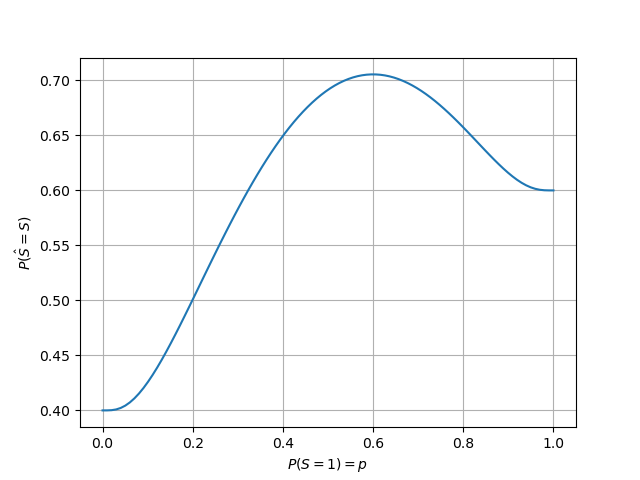
\includegraphics[width=0.8\linewidth]{elec-decoding-errors.png}
\caption{$\mathbb P(\hat S = S)$ for varying $p$.}
\end{figure}
